\documentclass[a4paper]{article}

\usepackage{amsmath}
\usepackage{tabularx}
\usepackage{todonotes}
%\usepackage{showframe}
\begin{document}

%\title{Title}
%\author{Author}
%\date{Today}
%\maketitle



\section{Organization and Introduction}
\begin{itemize}
\item The Art of managing complexity
\begin{itemize}
\item Abstraction: Hiding details when they are not important
\item Discipline: Intentionally restricting your design choices to that you can work more productively at higher abstraction levels
\item The three -Y's
\begin{itemize}
\item Hierarchy: A system is divided into modules of smaller complexity
\item Modularity: Having well defined functions and interfaces
\item Regularity: Encouraging uniformity, so modules can be easily re-used
\end{itemize}
\end{itemize}
\item Bit: \textbf{B}inary dig\textbf{it}
\end{itemize}

\section{Binary Numbers}
\begin{itemize}
\item Powers of two:\\
\begin{tabular}{c|c|c}
$2^0= 1$ & $2^5=32$ & $2^{10}= 1024$\\ 
$2^1= 2$ & $2^6=64$ & $2^{11}= 2048$\\ 
$2^2= 4$ & $2^7=128$ & $2^{12}= 4096$\\ 
$2^3= 8$ & $2^8=256$ & $2^{13}= 8192$\\ 
$2^4= 16$ & $2^9=512$ & $2^{14}= 16384$\\ 
\end{tabular}
\item Binary to decimal conversion
\begin{align*}
10011_2&=2^4\times 1 +2^3\times 0 + 2^2\times 0 +2^1\times 1 +2^0\times 1\\
&=16 \times 1+8 \times 0+4 \times 0+2 \times 1+1 \times 1\\
&=16+0+0+2+1=19_{10}
\end{align*}
\item Convert decimal to binary (roughly). Example with $47_{10}$ to binary\\
\begin{tabular}{c|c|c|c|c}
$2^6=64$& is $64\leq 47$?&no&0&do nothing\\ 
$2^5=32$& is $32\leq 47$?&yes&1&47-32=15\\
$2^4=16$& is $16\leq 15$?&no&0&do nothing\\
$2^3=8$& is $8\leq 15$?&yes&1&15-8=7\\ 
$2^2=4$& is $4\leq 7$?&yes&1&7-4=3\\
$2^1=2$& is $2\leq 3$?&yes&1&3-2=1\\
$2^0=1$& is $1\leq 1$?&yes&1&1-1=0; done!\\
\end{tabular}\\
$\Rightarrow 47_{10}$ to binary is $0101111_2$ 
\item Binary values and range
\begin{itemize}
\item $N-$digit decimal number
\begin{itemize}
\item How many values: $10^N$
\item Range: $\lbrack 0,10^{N}-1\rbrack$
\item Example (3-digit number): $10^3=1000$ possible values, range:$\lbrack 0,999\rbrack$
\end{itemize}
\item $N-$bit binary number
\begin{itemize}
\item How many values: $2^N$
\item Range: $\lbrack 0,2^{N}-1\rbrack$
\item Example (3-digit number): $2^3=8$ possible values, range:$\lbrack 0,7\rbrack=\lbrack 000_2\text{ to }111_2\rbrack$
\end{itemize}
\end{itemize}
\item Hexadecimal (Base-16) Numbers\\
\begin{tabular}{c|c|c|c|c|c|c}
Decimal & Hexadecimal & Binary&{}&Decimal & Hexadecimal & Binary\\\hline
0&0&0000&{}&8&8&1000\\
1&1&0001&{}&9&9&1001\\
2&2&0010&{}&10&A&1010\\
3&3&0011&{}&11&B&1011\\
4&4&0100&{}&12&C&1100\\
5&5&0101&{}&13&D&1101\\
6&6&0110&{}&14&E&1110\\
7&7&0111&{}&15&F&1111\\
\end{tabular}
\item Bits, Bytes, Nibbles...
\[\begin{array}{*{20}{c}}
{\underbrace 1_{{\text{MSB}}}001011\underbrace 0_{{\text{LSB}}}}&{\overbrace {1001\underbrace {0110}_{{\text{nibble}}}}^{{\text{Byte}}}}&{\underbrace {{\text{CE}}}_{{\text{MSB}}}{\text{BF9A}}\underbrace {{\text{D7}}}_{{\text{LSB}}}}
\end{array}\]
Where MSB=Most significant Bit and LSB=Least significant Bit
\item Addition in base two works exactly the same as in base 10, using carries
\item Overflow
\begin{itemize}
\item Digital systems operate on a fixed number of bits
\item Addition overflows when the result is too big to fit in the available number of bits
\end{itemize}
\item Signed Binary Numbers
\begin{itemize}
\item Sign/Magnitude Numbers
\begin{itemize}
\item 1 sign bit, $N-1$ magnitude bits
\item Sign bit is the most significant (left-most) bit
\item Example: 4-bit sign/mag repr. of $\pm 6$:
\begin{itemize}
\item $+6=\textbf{0}110$
\item $-6=\textbf{1}110$
\end{itemize}
\item Range of an $N-$bit sign/magnitude number:\\
$\lbrack -\left( 2^{N-1}-1\right),2^{N-1}-1\rbrack$
\item Problems:
\begin{itemize}
\item Addition doesn't work
\item Two representations of 0 ($\pm 0$): 1000 and 0000
\item Introduces complexity in the processor design
\end{itemize}
\end{itemize}
\item One's Complement Numbers
\begin{itemize}
\item A negative number is formed by reversing the bits of the positive number (MSB still indicates the sign of the integer)\\
\begin{tabular}{|c|c|c|c|c|c|c|c|c|c|c|}
\hline
$2^7$&$2^6$&$2^5$&$2^4$&$2^3$&$2^2$&$2^1$&$2^0$&{}&One's Compl.&Unsigned\\\hline\hline
0&0&0&0&0&0&0&0&$=$&0&0\\
0&0&0&0&0&0&0&1&$=$&1&1\\
0&0&0&0&0&0&1&0&$=$&2&2\\
\dots&\dots&\dots&\dots&\dots&\dots&\dots&\dots&\dots&\dots&\dots\\
0&1&1&1&1&1&1&1&$=$&127&127\\
1&0&0&0&0&0&0&0&$=$&-127&128\\
1&0&0&0&0&0&0&1&$=$&-126&129\\
\dots&\dots&\dots&\dots&\dots&\dots&\dots&\dots&\dots&\dots&\dots\\
1&1&1&1&1&1&0&1&$=$&-2&253\\
1&1&1&1&1&1&1&0&$=$&-1&254\\
1&1&1&1&1&1&1&1&$=$&-0&255\\\hline
\end{tabular}
\item Range of $n-$bit number: $\lbrack -2^{n-1}-1,2^{n-1}-1\rbrack$, 8 bits:$\lbrack -127,127\rbrack$
\item Addition: Done using binary addition with end-around carry. If there is a carry out of the MSB of the sum, this bit must be added to the LSB of the sum
\end{itemize}
\item Two's Complement Numbers
\begin{itemize}
\item Don't have same problems as sign/magnitude numbers:
\begin{itemize}
\item addition works
\item Single representation for 0
\end{itemize}
\item Has advantages over one's complement:
\begin{itemize}
\item Has a single 0 representation
\item Eliminates the end-around carry operation required in one's complement addition.
\end{itemize}

\item A negative number is formed by reversing the bits of the positive number (MSB still indicates the sign of the integer) and adding 1:\\
\begin{tabular}{|c|c|c|c|c|c|c|c|c|c|c|}
\hline
$2^7$&$2^6$&$2^5$&$2^4$&$2^3$&$2^2$&$2^1$&$2^0$&{}&Two's Compl.&Unsigned\\\hline\hline
0&0&0&0&0&0&0&0&$=$&0&0\\
0&0&0&0&0&0&0&1&$=$&1&1\\
0&0&0&0&0&0&1&0&$=$&2&2\\
\dots&\dots&\dots&\dots&\dots&\dots&\dots&\dots&\dots&\dots&\dots\\
0&1&1&1&1&1&1&1&$=$&127&127\\
1&0&0&0&0&0&0&0&$=$&-128&128\\
1&0&0&0&0&0&0&1&$=$&-127&129\\
\dots&\dots&\dots&\dots&\dots&\dots&\dots&\dots&\dots&\dots&\dots\\
1&1&1&1&1&1&0&1&$=$&-3&253\\
1&1&1&1&1&1&1&0&$=$&-2&254\\
1&1&1&1&1&1&1&1&$=$&-1&255\\\hline
\end{tabular}
\item Same as unsigned binary, but the most significant bit (MSB) has value of $-2^{N-1}$
\begin{itemize}
\item Most positive 4-bit number: 0111
\item Most negative 4-bit number: 1000
\end{itemize}
\item The most significant bit still indicates the sign (1=neg., 0=pos.)
\item Range of an $N-$bit two's comp. number: $\lbrack -2^{N-1},2^{N-1}-1\rbrack$, 8 bits:$\lbrack -128,127\rbrack$
\end{itemize}
\end{itemize}
\item Increasing bit width (assume from $N$ to $M$, with $M>N$): 
\begin{itemize}
\item Sign-extension
\begin{itemize}
\item Sign bit is copied into MSB
\item Number value remains the same
\item Give correct result for two's compl. numbers
\item Example 1:
\begin{itemize}
\item 4-bit representation of $3=\textbf{0}011$
\item 8-bit sign-extended value: $\textbf{00000}011$
\end{itemize}
\item Example 2:
\begin{itemize}
\item 4-bit representation of $-5=\textbf{1}011$
\item 8-bit sign-extended value: $\textbf{11111}011$
\end{itemize}
\end{itemize}
\item Zero-extension
\begin{itemize}
\item Zeros are copied into MSB
\item Value will change for negative numbers
\item Example 1:
\begin{itemize}
\item 4-bit value: $0011_2=3_{10}$
\item 8-bit zero-extended value: $\textbf{0000}0011_2=3_{10}$
\end{itemize}
\item Example 2:
\begin{itemize}
\item 4-bit value: $1011_2=-5_{10}$
\item 8-bit zero-extended value: $\textbf{0000}1011_2=\textbf{$11_{\textbf{10}}$}$
\end{itemize}
\end{itemize}
\end{itemize}
\end{itemize}

\section{Short Introduction to Electrical Engineering (EE Perspective)}
\begin{itemize}
\item The goal of circuit design is to optimize:
\begin{itemize}
\item Area: Net circuit area is proportional to the cost of the device
\item Speed/Throughput: We want circuits that work  faster, or do more
\item Power/Energy
\begin{itemize}
\item Mobile devices need to work with a limited power supply
\item High performance devices dissipate more than 100W/$cm^2$
\end{itemize}
\item Design time
\begin{itemize}
\item Designers are expensive
\item The competition will not wait for you
\end{itemize}
\end{itemize}
\item (Frank's) Principles for engineering
\begin{itemize}
\item Good engineers are lazy: They do not want to work unnecessarily, be creative
\item They know how to ask the question ``why''?: take nothing for granted
\item Engineering is not a religion: Use what works best for you
\item Keep it simple and stupid: Engineers' job is to manage complexity
\end{itemize}
\item Building blocks for microchips
\begin{itemize}
\item Conductors: Metals (Aluminium, Copper)
\item Insulators: Glass (SiO$_2$), Air
\item Semiconductors: Silicon (Si), Germanium (Ge)
\end{itemize}
\item N-type Doping: Add extra electron (negatively charged), zone becomes negatively charged\todo{Maybe add a definition or a better explanation}
\item P-type Doping: Remove electron, zone becomes positively charged
\item Semiconductors:
\begin{itemize}
\item You can ``Engineer'' its properties, i.e.
\begin{itemize}
\item Make it P type by injecting type-III elements (b, Ga, In)
\item Make it N type by injecting elements from type-V (P, As)
\end{itemize}
\item You can combine P and N regions to each other, from a pure semiconductor
\item Allows you to make interesting electrical devices (Diodes, Transistors, Thrystors)
\end{itemize}
\item pMOS is a P type transistor, nMOS an N type transistors; combined they are a CMOS
\item CMOS (Properties)
\begin{itemize}
\item No input current: Capacitive input, no resistive path from the input
\item No current when output is at logic levels: Little static power, current is needed only when switching
\item Electrical properties determined directly by geometry: A transistor that is 2 times larger drives twice the current
\item Very simple to manufacture: pMOS and nMOS can be manufactures on the same substrate
\end{itemize}
\item CMOS Gate Structure
\begin{itemize}
\item The general form used to construct any inverting logic, such as: NOT, NAND, NOR
\begin{itemize}
\item The networks may consist of transistors in series or parallel
\item When transistors are in parallel, the network is ON if either transistor is ON
\item When transistors are in series, the network is ON only if all transistors are ON
\end{itemize}
\item In a proper logic gate: One of the networks should be ON and the other OFF at any given time
\item Use the rule of conduction complements:
\begin{itemize}
\item When nMOS transistors are in series, the pMOS transistor must be in parallel
\item When nMOS transistors are in parallel, the pMOS transistors must be in series
\end{itemize}
\end{itemize}
\todo[inline]{Add picture on slide 34, 03 - EEPerspective}
\item Logic Gates
\begin{itemize}
\item Perform logic functions: Inversion (NOT), AND, OR, NAND, NOR, etc.
\item Single input: NOT gate, buffer
\item Two-input: AND, OR, XOR, NAND, NOR, XNOR\\
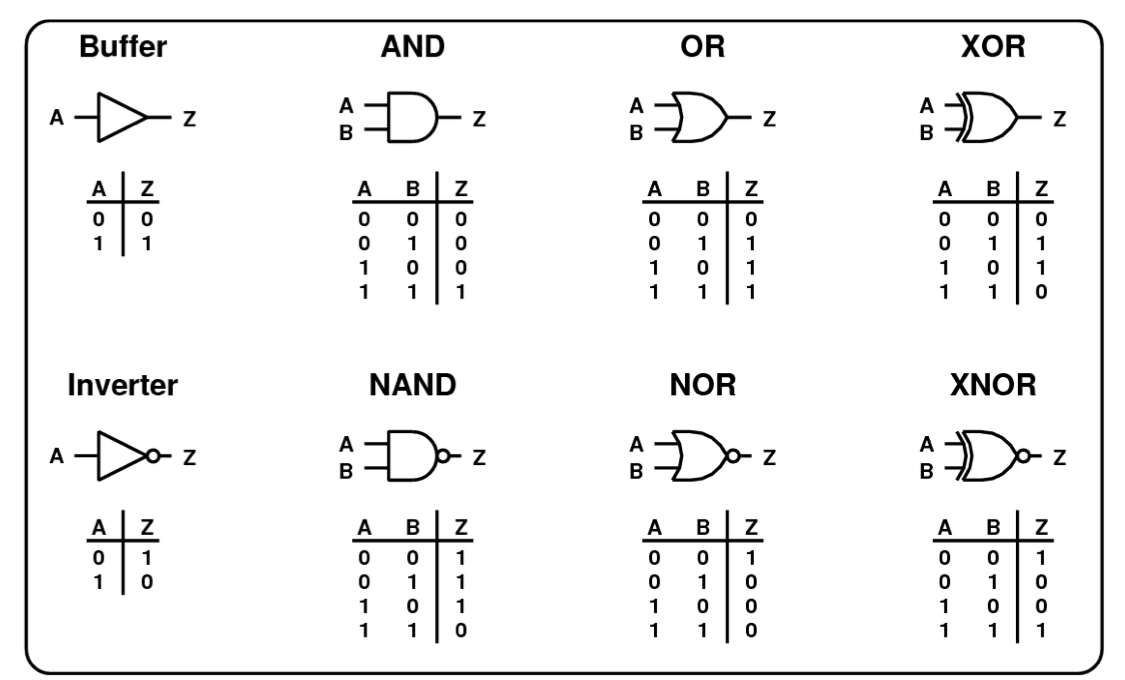
\includegraphics[scale=0.27]{Figures/commonLogicGates.jpg}
\item Multiple-Input:
\begin{itemize}
\item 3, 4, or even more input AND, OR, XOR gates
\item Compound gates
\begin{itemize}
\item AND-OR
\item OR-AND
\item AND-OR-INVERT
\item OR-AND-INVERT
\end{itemize}
\item Other cells: Multiplexers and Adders
\end{itemize}
\end{itemize}
\item Logic Levels
\begin{itemize}
\item Define ranges of discrete voltages to represent 1 and 0 (i.e. 0 for ground and 1 for 5V ($V_{DD}$)) and allow for noise.
\end{itemize}
\item Noise: Is anything that degrades the signal (i.e. resistance, power supply noise, etc.)
\item Moore's Law
\begin{itemize}
\item \emph{``Number of transistors that can be manufactured doubles roughly every 18 months.''} - Gordon Moore, 1965
\end{itemize}
\item How do we keep Moore's Law:
\begin{itemize}
\item Manufacturing smaller structures: some structures are already a few atoms in size
\item Developing materials with better properties
\item Optimizing the manufacturing steps
\item New technologies
\end{itemize}
\item Power consumption
\begin{itemize}
\item Power = Energy consumed per unit time
\item Two types of power consumption:
\begin{enumerate}
\item Dynamic power consumption: Power to charge transistor gate capacitances \[P_{\text{dynamic}}=\frac{1}{2}CV_{DD}^2f\]
\item Static power consumption: Power consumed when no gates are switching, caused by the leakage current \[P_{\text{static}}=I_{DD}V_{DD}\]
\end{enumerate}
\end{itemize}
\end{itemize}

\section{Combinational Circuits: Theory}
\begin{itemize}
\item Circuit elements. A circuit consists of:
\begin{itemize}
\item Inputs
\item Outputs
\item Nodes (wires): Connections between I/O and circuit elements. To count them, look at
\begin{itemize}
\item Outputs of every circuit elements
\item Inputs to the entire circuit
\end{itemize}
\item Circuit elements
\end{itemize}
\item Types of Logic Circuits
\begin{itemize}
\item Combinational Logic
\begin{itemize}
\item Memoryless
\item Outputs determined by current values of inputs
\item In some books called Combinatorial Logic
\end{itemize}
\item Sequential Logic
\begin{itemize}
\item Has Memory
\item Outputs determined by previous and current values of inputs
\end{itemize}
\end{itemize}
\item Rules of Combinational Composition
\begin{itemize}
\item Every circuit element is itself combinational
\item Every node of the circuit is either
\begin{itemize}
\item Designated as an input to the circuit
\item Connects to exactly one output terminal of a circuit element
\end{itemize}
\item The circuit contains no cyclic paths: Every path through the circuit visits each node at most once
\item Boolean Equations\footnote{For a more in depth look, use the material from Diskrete Mathematik}
\end{itemize}

\end{itemize}
\end{document}